\documentclass[a4paper,12pt]{article}
\usepackage[hidelinks]{hyperref}
\usepackage{graphicx}
\usepackage{float}
\usepackage{caption}
\begin{document}
\begin{center}

%Cover page
\Huge\textbf{Functional Requirements(uWatch digital forensic tool)\\}
																											
\vspace{2 cm}

\LARGE\textbf{Group Name:} MPHETamines\newline
 
 
 
 
 
\vspace{0.5 cm}
\begin{tabular}{lr}
Taariq Ghoord&10132806
\\ 
Martha Mohlala&10353403
\\
Phethile Mkhabela&12097561
\\
Sboniso Masilela&%Enter student number
\\
Harrison Maphuti Setati&12310043\\
\end{tabular}

\vspace{1cm}
\textbf{Git repository link:\\}
\url{https://github.com/MPHETamines/MPHETamines/}

\vspace{1cm}
\textbf{Date:} 20 May 2015
\end{center}
\pagenumbering{gobble}
\newpage

%table of contents
\tableofcontents







\newpage
\pagenumbering{arabic}

\section{Introduction}

Crime is a prominent issue in South Africa as it is all over the world, Many criminal activities go unresolved or even attended to due to the lack of evidence or concrete witnesses.  Mobile applications have become increasingly popular all over the world and are used in our everyday and work life for common things such as checking the weather; maps for directions and news feed updates.  Digital forensic science hopes to utilise this increasing growth in the use of mobile applications to address the lack of evidence to crime cases in South Africa.
The application is referred to as online neighbourhood watch(ONW) accessible via mobile devices and computers over the internet.  The two main users of the ONW model are the uploader (user of the mobile device) and the forensic investigator or law enforcement agent. 
This tool is to be used by the citizens of South Africa to capture, collect and store potential evidence which can later be viewed and analysed by the Police department and used in the prosecution and detention of criminals.
\subsection{Purpose}
[Provide an overall description of the FRD, its purpose.  Reference the system name and identifying information about the system to be implemented.]
\subsection{Scope}
[Discuss the scope of the document and how it accomplishes its purpose.]
\subsection{Background}
[Describe the organization and its overall responsibilities.  Describe who is producing the document and why.]
\subsection{References}
[List references and controlling documents, including: meeting summaries, white papers, other deliverables, etc.]
\subsection{Assumptions and Constraints}
[Provide a list of contractual or task level assumptions and/or constraints that are preconditions to preparation of the FRD.  Assumptions are future situations beyond the control of the project, whose outcomes influence the success of a project.]
\subsubsection{Assumptions}
Examples of assumptions include: availability of a technical platform, legal changes and policy decisions. 
\subsubsection{Constraints}
Constraints are boundary conditions on how the system must be designed and constructed.  Examples include: legal requirements, technical standards, strategic decisions. 
•	Constraints exist because of real business conditions.  For example, a delivery date is a constraint only if there are real business consequences that will happen as a result of not meeting the date.  If failing to have the subject application operational by the specified date places the organization in legal default, the date is a constraint.
•	Preferences are arbitrary.  For example, a date chosen arbitrarily is a preference.  Preferences, if included in the FRD, should be noted as such.]%%%This is important


\subsection{Document Overview}
[Provide a description of the document organization.]



\section{Methodology}
[Describe the overall approach used in the determination of the FRD contents.  Describe the modeling method(s) so non-technical readers can understand what they are conveying.]

\section{Functional Requirements}
\subsection{Context}
[Provide a context diagram of the system, with explanations as applicable.  The context of a system refers to the connections and relationships between the system and its environment.]

\subsection{User Requirements}
[Provide requirements of the system, user or business, taking into account all major classes/categories of users.  Provide the type of security or other distinguishing characteristics of each set of users.  List the functional requirements that compose each user requirement.  As the functional requirements are decomposed, the highest level functional requirements are traced to the user requirements.  Inclusion of lower level functional requirements is not mandatory in the traceability to user requirements if the parent requirements are already traced to them.
User requirement information can be in text or process flow format for each major user class that shows what inputs will initiate the system functions, system interactions, and what outputs are expected to be generated by the system.  The scenarios should be comprehensive, to the extent that all user types and all major functions are covered.  Give each user requirement a unique number.  Typically, user requirements have a numbering system that is separate from the functional requirements.  Requirements may be labeled with a leading “U” or other label indicating user requirements.]


\subsection{Use Case Diagrams}

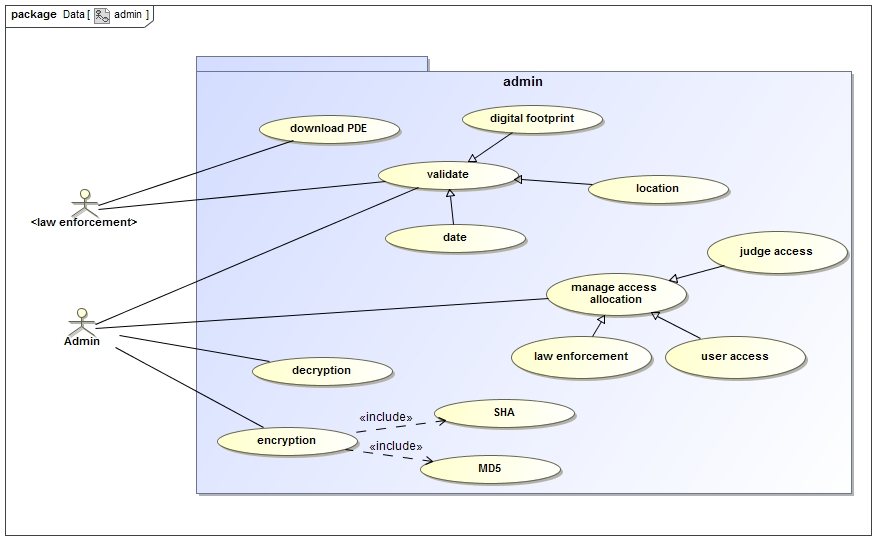
\includegraphics[width=1.0\textwidth]{images/admin.jpg}
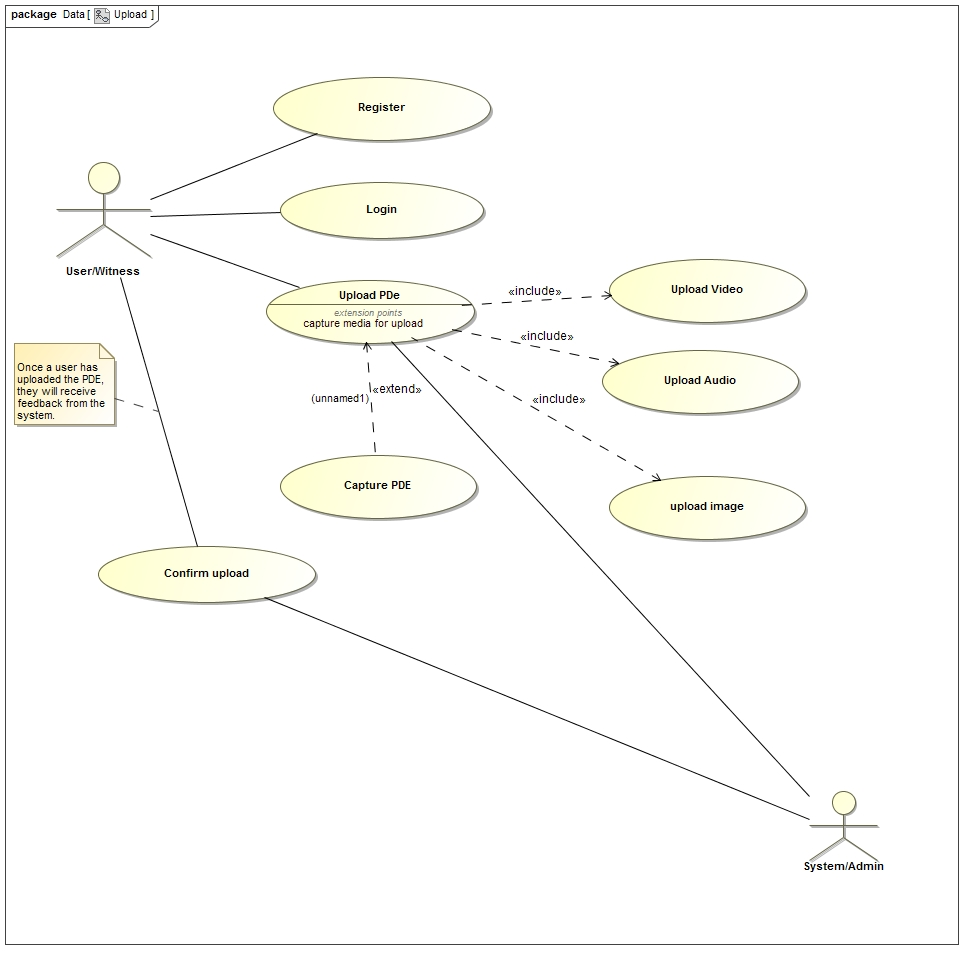
\includegraphics[width=1.0\textwidth]{images/upload.jpg}
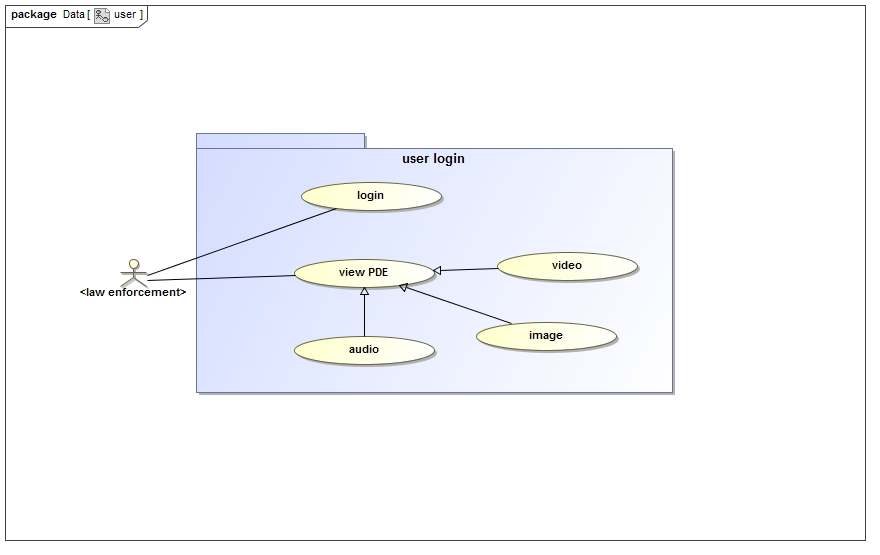
\includegraphics[width=1.0\textwidth]{images/user.jpg}

\subsection{Class And Sequence Diagrams}
[service contracts and their corresponding sequence diagrams to be shown here]

\subsection{Activity Diagrams}
[flow of the system in different contexts]

\subsection{Functional Requirements}
[List the functional requirements of the system.]

\end{document}
